\newcommand{\f}[1]{\textsf{#1}\xspace}

\newcommand{\flanguage}{\f{Language}}

\newcommand{\feditor}{\f{Editor}}
\newcommand{\fsimulator}{\f{Simulator}}
\newcommand{\fdebugging}{\f{Debugging}}
\newcommand{\fspectime}{\f{SpecificationTime}}
\newcommand{\fdeployment}{\f{MissionDeployment}}
\newcommand{\fmultilang}{\f{MultiLanguageSupport}}


\newcommand{\fsemantics}{\f{Semantics}}
\newcommand{\fnotation}{\f{Notation}}
\newcommand{\flangparadigm}{\f{LanguageParadigm}}
\newcommand{\fextensibility}{\f{Extensibility}}

\newcommand{\flangconcepts}{\f{LanguageConcepts}}


\newcommand{\fflowchart}{\f{FlowChart}}
\newcommand{\fblockly}{\f{Blockly}}


\section {Analysis of Identified Environments - RQ2}

\Figref{fig:featuremodel} shows the general structure of the features we identified in our environments. 
We classified the key, top-level features into (\secref{sec:envfeatures}) capabilities and characteristics of the environments, represented by the features \feditor, \fsimulator, \fdebugging, \fspectime, \fdeployment, and \fmultilang; into (\secref{sec:langcharacteristics}) general language characteristics, represented by the feature \flanguage; and into (\secref{sec:langconcepts}) the actual concepts the languages offer to specify missions, represented by the feature \flangconcepts.
%\claudio{
%How many features have been identified in total? How many optional etc?
%How many features were identified in he brainstorming meeting? How many features were extracted from other sources?}
%\claudio{What is a general language feature? what is a Language concept?}
%\claudio{What are you going to discuss in the next two sections?}


\subsection{Specification Environment}\label{sec:envfeatures}
\noindent
We identified the following distinguishing environment characteristics that are related to the specification of missions.
%The value in brackets indicates the number of environments offering the optional feature out of 29. While simulator (10/29), multiLanguageSupport (13/29) and debugging (13/29) features are optional. Much as it is desirable to have to have a debugger and a simulator, not all the environments supported these features. 

\begin{figure}[t]
     \centering
    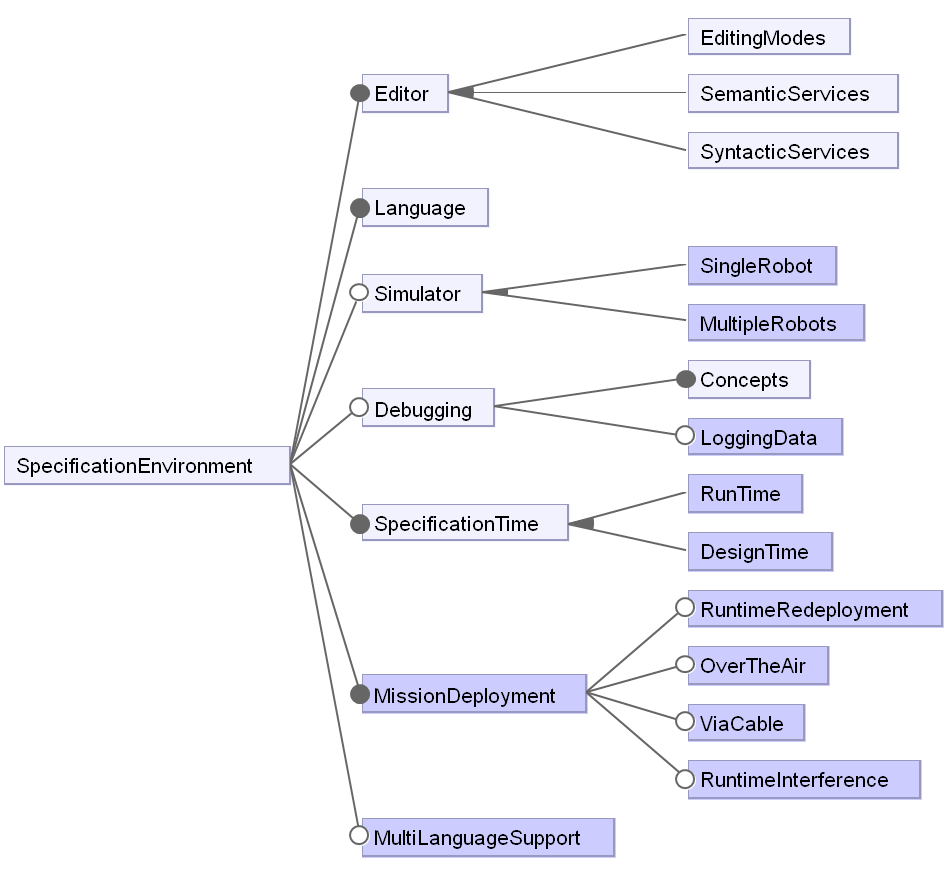
\includegraphics[width=\columnwidth]{fig/toplevelfeatures.png}
		  \smash{\begin{minipage}{8.3cm}
						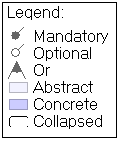
\includegraphics[width=.18\columnwidth]{fig/legend.png}
						\vspace{2.3cm}
						\end{minipage}
			}
			\vspace{-.3cm}
      \caption{Overview of all features identified%\tb{was my version, please update, but please fix the naming of some features as I did in this figure}
      }
      \label{fig:featuremodel}
			\vspace{-.4cm}
\end{figure}

\newcommand{\fsyntacticservices}{\f{SyntacticServices}}
\newcommand{\fsemanticservices}{\f{SemanticServices}}
\newcommand{\feditingmode}{\f{EditingMode}}

\parhead{\feditor.} While the editor tooling in our environments of course offers typical editor capabilities (e.g., copy, paste or undo), we found the following distinguishing characteristics represented by the features \fsyntacticservices, \fsemanticservices, and \feditingmode, as follows.

%Besides the basic editor features such as cut, paste, and redo; we also found syntactic services, semantic services, and editing modes as editor features.

Syntactic services (feature \fsyntacticservices) support developers creating a correct abstract syntax tree (AST) of the mission specification, according to the language's abstract syntax. We found various of such services. Especially syntax highlighting with coloring is available in all environments.  %todo: verify \flyaq and \tivipe
We furthermore found a range of convenience services, such as an outline view for navigation support (e.g., in \picaxe), syntactic completion templates for users (e.g., in \edison and \ardublockly), and automated formatting (e.g., in \arcbotics, \robotmesh, and \vex).

%and invalid variable name \minibloq -> isn't that a kind of error highlighting?

%restructuring, aligning or lay-outing \cite{erdweg2013languageworkbenches} as seen in \robotmesh, \vex  -> explain what that is (didn't find in the spreadsheet)

%offer support for correct expression structure, as defined by a language to support specification of missions. The syntactic services captured include; language specific syntax coloring and symbol shapes in graphical notations, were evident in almost all the environments studied with exception of \flyaq and \tivipe where the authors were not sure. -> symbol shapes is not a syntactic service

Semantic services (feature \fsemanticservices) support developers creating an abstract syntax tree that is semantically meaningful, inspired by the definition of semantic services in~\citet{erdweg2013languageworkbenches}. We identified: auto-completion (e.g., in \vex, \trik, \picaxe, \edison);  live translation where generated code is displayed side-by-side to the graphical notation (e.g., in \easyc); error highlighting (e.g., in \edison, \aseba, \vex, \robotmesh, \blocklyprop, \minibloq, and \easyc) directly on the mission specification, for instance the indication of compile errors at the respective lines in \blocklyprop, or as a pop-up help (e.g., in \edison, \missionlab, and \choregraphe). However, more than half of the environments did not offer any semantic services. % -> verify

%and auto-help when activated enables automatic reference when blocks are selected ~\cite{ozobot} as seen in \ozoblockly, \edison.

Finally, the editing mode (feature \feditingmode) typically classifies into parser-based and projectional editing\,\cite{voelter2014projectional,berger2016pe}. In the former, the user edits the source code, which is represented by a sequence of characters in a free form. In the latter, the user's editing gestures directly change the underlying AST, which is projected using projection rules into a user-observable syntax, which can resemble textual and visual syntax, or a combination of both. \Figref{fig:easyc-sidebyside} illustrates the power of projectional editing in the environment \easyc, showing visual and textual syntax side-by-side. The typical continuous enforcement of a correct AST in projectional editing guides users towards correct mission specifications, which can also be seen as a semantic service. For all our environments, given the restriction to visual languages, every environment provides a projectional editor. However, three also offer textual languages, to be used in parallel as an alternative, relying on parser-based editing: \aseba, \vex, and \turtlebot.% and \robotc\tb{where is that stated for \robotc? can you give me the exact source?}.

\parhead{\fmultilang.} A total of 13 of our environments offer multiple languages to specify missions. While at least one visual language is supported (according to our selection criteria), many environments offer at least one more language. For instance, \picaxe provides two visual languages, based on a \fflowchart and a \fblockly notation, respectively, as well as it offers a language with a textual syntax in the style of the programming language Basic, as well as it offers the use of JavaScript.


%, and projectional mode where, the program has a standard fixed layout. In projectional editors are structured editors in which a developer works directly on the bstract syntax tree(AST) \cite{berger2016pe}, coding is done using intuitive onscreen visuals.
%\parheadit{Example} Of the 29 environment studied, only four support parser based editing mode; \aseba, \vex, \turtlebot and \robotc. This finding is not surprising since in the selection criteria, the study is biased to end-user supporting environments. 

\parhead{\fsimulator.} Ten of our environments provide simulation support to test missions before they are executed. This helps in ensuring safety and creating opportunities to train users without necessarily using the actual robots. One of the simulators, that of \missionlab, even supports multiple robots.
%The simulator either support single robot at a time or more than one robot and/or robot type. -> which ones? do we have evidence that multiple robots are supported by at least one simulator?

\parhead{\fdebugging.} A total of 13 of our environments offer debugging support. We found a variety of debugging tools, including the live monitoring of sensor data, the state of actuators, and variables in the environments \picaxe, \aseba, \trik, \flyaq, \easyc, and \edison. The environment \edison offers a box to control inputs, manipulate data, and monitor the use of variables. % -> what was 'bug-box'?
Interestingly, \makecode communicates execution traces via sound and printing text between the execution of program blocks. % -> not so clear
We also found the typical break-point mechanism to hold and monitoring executions (e.g., in \robotmesh).
Furthermore, \openroberta provides a 'check' menu\tb{please give me the exact source of this information (paper and position)} to confirm that the mission specification the robot's configuration matches---important since the environment supports different types of robots. 
% -> this all needs to be verified

\parhead{\fspectime.} Missions are specified either at design time or run-time. Design-time specification provides all the details about the mission before the execution starts.
 %which calls for explicit modeling of the environment.
All our environments support design-time specification. A few environments (\turtlebot, \sphero, and \choregraphe), however, also offer some remote-control functionality to intercept the mission execution at runtime. % -> verify
%with the exception of \turtlebot, \sphero and \choregraphe. For instance, in \choregraphe, different missions can be deployed on the robot at run-time. \sphero supports interaction with the robot at run-time using a Bluetooth connection. % -> I think this is wrong

\parhead{\fdeployment.} Missions, once specified, are transferred to the robots for execution. Not surprisingly, we found different combinations of media to transfer missions, including USB cable, Ethernet cable, custom cable, as well as WiFi and Bluetooth connections.
 %Environments such as \trik and \lego support USB, WiFi, and Bluetooth connections for deployment over-the-air. While \tello missions can be deployed using Bluetooth, and Wi-Fi. Most environments use either USB, Ethernet or a custom cable to deploy missions to robots. \\ 


% \textbf{items removed}
% \begin{itemize}
%     %\item file access
%     \item time has been merged as a measure of action under action types
%     \item example as an example of syntax services
%     \item formal notation (generic code, natural language text, forms, blocks, icons) and secondary notation (syntax highlighting, size, notation color, comments) as concrete features of notation.
%     \item behavior concepts with concrete features like discrete behavior and continuous behavior from language features
%     \item robot with single/multi-robot mission (swarm/team), multi-robot, single robot, robot types and connection and multi-robot types as concrete features
%     \item Mission deployment support; hardware requirements and software requirements
%     \item debugging environments; simulation, actual robot
%     \item modeling concepts and explicit modeling of environment 
% \end{itemize}





	
\subsection{General Language Characteristics}\label{sec:langcharacteristics}
As illustrated in \figref{fig:languagefeatures}, we identified the following general characteristics in which the languages differ, represented by the features: \fnotation, \fsemantics, \flangparadigm, and \fextensibility. The actual concepts offered by the languages will be discussed in \secref{sec:langconcepts}.

%The language constructs for motor, and sensor  data configurations are abstracted closer to those who are familiar to the use of the sensor than just robot engineers. For example \emph{set motor speed, obstacle detector event block (grey: ignore detector, white: object close and black: object far)}. \claudio{The previous sentences are part of the methodology} The fact that these languages support graphical notations breaks the barrier created by text notation among novice programmers, as asserted by Fernandez-Permomo et al.\cite{Fernandez-Perdomo2010}, hence increasing usability, learnability and satisfaction among end-users. \claudio{Not clear what is the point of this sentence? Here we should discuss the FM we have created}
%\tb{we need examples of domain-specific terminology in the languages, can you provide some? also, examples why you think the languages are end-user facing; why is that the case?}
%For instance, they support end users through \dots. Most (X\,\%) are also graphical.
%domain, which generalized features that support novice programmers and robotics domain, which take care of technical features for professionals in robotics or software engineering.
All the languages identified in the environments including the textual ones have been customized to support the robotics domain, for example by introducing domain specific actions. Some of the actions in \lego are stop motors, play tone in \trik, set robot's state, set top color in \aseba,  drive straight, and turn right. %in \lego are some domain specific actions.% \tb{how? give examples of domain-specific keywords and domain-specific graphical elements}.

\begin{figure}[t]
     \centering
    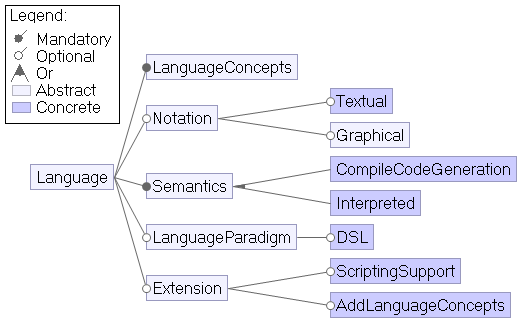
\includegraphics[width=\columnwidth]{Languagefeatures.png}
      \caption{Language Characteristics}
      \label{fig:languagefeatures}
   \end{figure}

\parhead{\fnotation.} All our environments offer languages with a domain-specific visual notation (concrete syntax) for end users. For instance, a block \emph{Motor forward} in \trik has a gear icon with a forward arrow depicting a forward-running motor. The user only specifies the motor power and the port in which the motor connects. 13 of our environments additionally offer a textual syntax

\tb{I think I now know how to write this part, will do later; got a lot of insights from looking through the data an the screenshots I took over the weekend}
%\tb{do you know for how many the textual syntax belongs to the same language (the main, visual language) and for how many it is a separate language (which could also be a gpl)?}.

\begin{itemize}
	\item Graph-based
	\item 
\end{itemize}

The notation found is: (i) Blockly-based as shown in Figure \ref{metabot}, (ii) Scratch-based as shown in Figure
	\ref{scratch-marty}, (iii) forms and tables as shown in Figure \ref{fig:robotcgraphical}, or (iv) textual where End-user codes a mission using text characters.

%\tb{but thought we have graph-based and block-based as our features?}
%\begin{itemize}
%	\item Blockly-based as shown in figure \ref{metabot}%\tb{characterize what you've seen; how does it look like}
%	\item Scratch-based as shown in figure
%	\ref{scratch-marty}%\tb{characterize what you've seen; how does it look like}
%	\item forms and tables as shown in figure \ref{fig:robotcgraphical}%\tb{characterize what you've seen; how does it look like}
%	\item textual where End-user codes a mission using text characters.%\tb{characterize what you've seen; what kinds of textual notations do we have? how do they look like?}
%\end{itemize}

Some of the graphical notations used blocks, which are directly connected to each other for instance \trik, blockly, and scratch based languages. While \choregraphe, Flowol in \robotmesh, and flowchat in \picaxe use connectors between blocks to form graph like structures. %A graphical notation is either block-based or graph-based. A block-based \tb{what's the difference? briefly describe}.
Interestingly, \flyaq offers a map-based 
%\tb{so, is that classified as graph-based or block-based, or sth. else?} 
monitoring mission language to specify missions by clicking on locations where tasks will be executed. 

The textual or visual notations offered by the respective environments are summarized in \tabref{notation}. Some environments use a mix of textual and visual notations, like \easyc, as shown in \figref{fig:easyc-sidebyside}, or make use of tables and forms, as \robotc as shown in  %\figref{fig:robotctextual} and 
\figref{fig:robotcgraphical}.

\aseba: \figref{fig:aseba-vpl}

\begin{figure}[b]
	\centering
	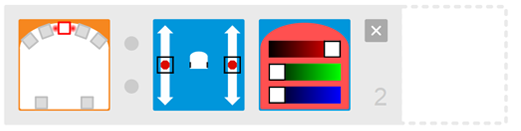
\includegraphics[width=\columnwidth]{fig/aseba-vpl-event-action-pairs.png}
	\caption{\aseba's visual notation for its language VPL, which is an event-based language consisting of event-action pairs. One such pair is shown here.}
	\label{fig:aseba-vpl}
\end{figure}


%Textual: \edison, \choregraphe, 
%%\tb{choregraphe is definitely visual!},\swaib{the point is it also supports textual notations} 
%visual: \minibloq, \trik, \choregraphe, and mix of both text and visual \easyc \figref{fig:easyc-sidebyside} or by use of tables and forms as provided by \robotc in  %\figref{fig:robotctextual} and 
%\figref{fig:robotcgraphical}. % \tb{add screenshot}.
%The notations offered by the respective environments have been summarized in the table \ref{notation}.

%- symbol shapes in graphical notations
%- Blockly library: It has been implemented in various environments as shown in table \ref{notation}% Roberta\,\cite{OpenRoberta,PICAXE,RobotMeshStudio} \tb{make complete, where else?}

\begin{figure}[t]
	\centering
	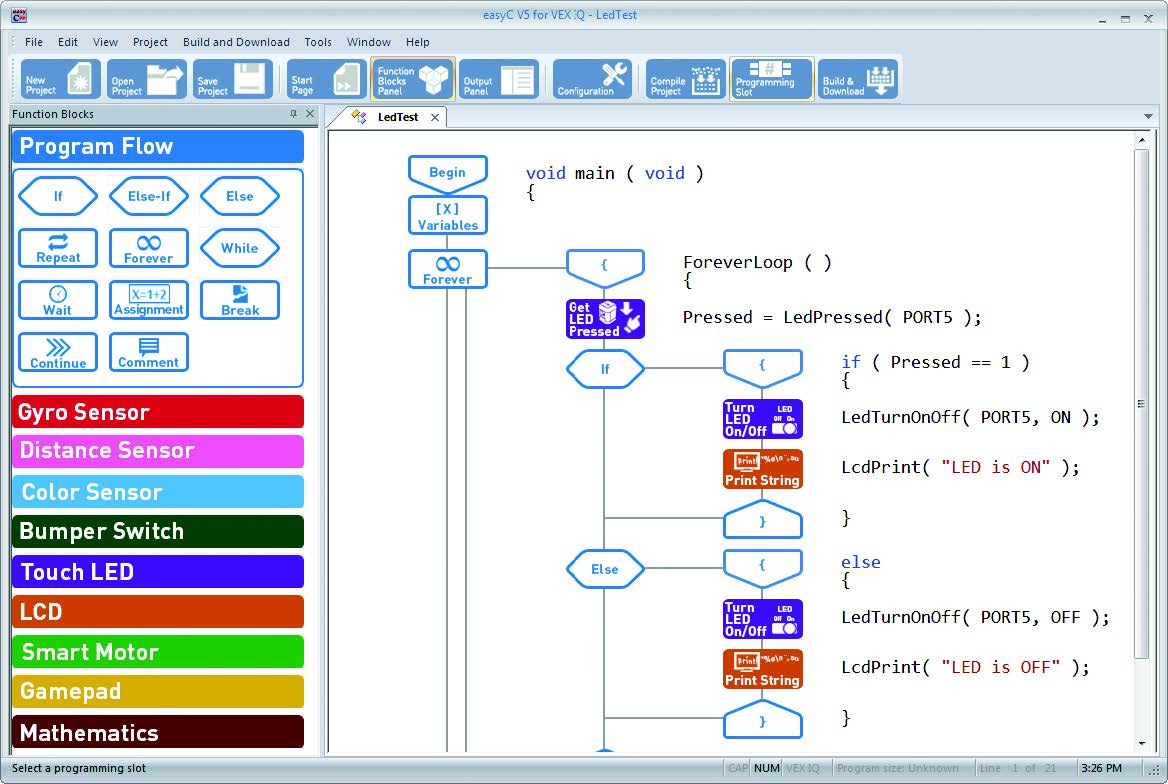
\includegraphics[max size={0.5\textwidth}{\textheight}]{projectionalEasyC.jpg}
	\caption{Graphical and textual syntax side-by-side in \easyc's projectional editor%\tb{TODO: create better screenshot}
	}\label{fig:easyc-sidebyside}
\end{figure}

% \begin{figure}[t]
% 	\centering
% 		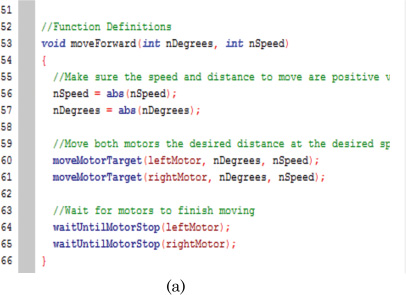
\includegraphics[max size={0.5\textwidth}{\textheight}]{robotCtext.png}
% 	\caption{RobotC, (a) textual \cite{Schunn2017} }
% 	\label{fig:robotctextual}
% \end{figure}

\begin{figure}[t]
	\centering
		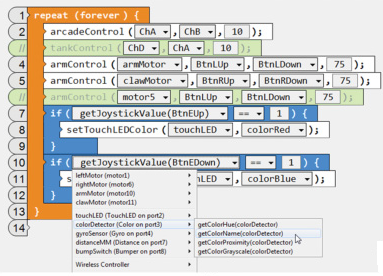
\includegraphics[width=\columnwidth]{robotCgraphical.png}	\caption{\robotc, graphical notation (from \cite{Schunn2017})\tb{quality too low; need a higher resolution image; actually, you write that you've installed it, so take a screenshot yourself (taking one yourself should always be done when possible, as opposed to copying from another paper (which requires saying explicitly 'from []' in the caption; this is also the only exception where you can refer directly to a [])}}
	\label{fig:robotcgraphical}
\end{figure}
%\claudio{Missing verb. Which details?} %Secondary notation services provide extra information on the marks and cues used for specification of missions, like; comments, and size of blocks~\cite{Blackwell2001}.

\begin{table*}
\caption{Kinds of notation supported by the environments (the graphical notations belongs to the primary DSLs of the environments; the textual ones to additional languages supported, which can be a GPL)}
\label{notation}
\begin{tabular}{ m{3cm}m{13.6cm}}
\toprule
\textsf{notation} &\textsf{environment}\\
\midrule
\textbf{graphical} &\\
Blockly-based & \picaxe, \ardublockly, \openroberta, \arcbotics, \aseba, \robotmesh, \blocklyprop, \ozoblockly, \turtlebot, \makecode, \robotc \\
Scratch-based & \edison, \aseba, \sphero, \vex (modkit), \marty, \makeblock, \codelab, \tello, \scratchev, \enchanting, \\
Control-flow graph & \picaxe (flow chart), \missionlab, \tivipe, \choregraphe (flow diagram), \robotmesh (flowol), \trik \\
Custom & \edison(EdBlock), \flyaq (map), \aseba(custom blocks with icons, see \figref{fig:aseba-vpl}), \codelab (icons), \lego(icons), \minibloq(icons), \easyc\\
\midrule
\textbf{textual}&\\
C/C++ & \arcbotics, \vex, \robotmesh, \trik, \easyc\\
Python & \edison, \robotmesh, \marty, \makeblock, \trik, \codelab\\
%Java & \patrizio{empty here? Remove?}\\
JavaScript & \picaxe, \sphero, \marty, \trik \\
Custom & \picaxe (custom language in the style of Basic), \ardublockly (Arduino C), \aseba (custom event-based language) \\
\bottomrule
\end{tabular}
\end{table*}



\parhead{\fsemantics} The semantics of our languages are determined by either interpretation or compilation (target code generation). The mission specified is either semantically translated (compiled) as shown in \tabref{Codegeneration} or interpreted to preserve what is specified and what the robot actually executes. Apart from \lego, and \codelab whose missions are interpreted, all the other 27 environments generate code. \metabot generates assembly code while the rest compile generated code before robot executes the mission.\patrizio{check this sentence. who are other? What do we want to say?}  \trik supports Lego Ev3, Lego NXT, pioneer kit, and the TRIK robot, even though the environment does not cross-compile as missions are robot specific. In the case of Lego EV3, missions are interpreted, with support for both USB and Bluetooth connections.
%\tb{this has nothing to do with semantics}. 
In the case of Lego NXT, besides interpretation, \trik generates Russian C language\tb{what is that? can you give me a reference to that language?} and NXT OSEK C language\tb{what is that? can you give me a reference?}, while in the case of TRIK robot, the environment generates Java Script, PascalABC, Python, and F\#.%\tb{why does it generate programs in so many different languages?} \swaib{Russian C, OSEK C are target languages seen in the list, however there is no much documentation about them in the tool documents. I have not figured out why TRI robot missions can be generated into several languages}. \codelab provides support for mission interpretation using Python SDK\tb{unclear, what does that mean?} \swaib{the interpreter was built using python software development kit (SDK)}.

% \begin{table*}
% \caption{Code generation matrix indicating languages of generated code from the graphical notations\tb{remove the classification according to the notation, just have a two-column table: first column: target language, second column: environment generating it; use the other tables' style}}
% \label{Codegeneration}
% \begin{tabular}{ |m{4em}|m{3cm}|m{2cm}|m{2cm}|m{3cm}|m{3cm}|}
% \hline
% \textbf{Graphical Notation} &\textbf{C/C++} &\textbf{Java} &\textbf{Java Script} &\textbf{Python}& \textbf{Others}\\
% \hline
% Blockly & \robotc, \blocklyprop, \robotmesh, \arcbotics, \openroberta  &\openroberta  & \openroberta, \makecode, \ozoblockly &\openroberta, \turtlebot, \robotmesh & \ardublockly (Arduino code), makebot (assembly code), \\
% \hline
% Scratch & &\enchanting, \scratchev, \vex & \sphero   & \tello, \makeblock, \marty & \\
% \hline
% State machine & \trik, \choregraphe, \missionlab &   &  \trik ,\choregraphe& \trik \choregraphe& \trik(F\#, PascalABC, NXT OSEK C), \choregraphe (Matlab, .NET), \picaxe(Basic) \\
% \hline
% Custom & \easyc, \minibloq, \tivipe & & &\edison &\flyaq(QBL), \aseba (VPL to Aseba event scripting language AESL) \\
% \hline

% \end{tabular}
% \end{table*}

\begin{table*}
\caption{Code generation matrix indicating the target generated language and the environments generating the code}
\vspace{-.4cm}
\label{tab:codegentable}
\begin{smaller}
\begin{tabular}{ m{2cm}m{14.6cm}}
\toprule
\textsf{Code Generation} &\textsf{Environment}\\
\midrule
%\textbf{graphical} &\\
C/C++ &  \robotc, \blocklyprop, \robotmesh, \arcbotics, \openroberta, \trik, \choregraphe, \easyc, \minibloq, \tivipe \\
Java & \openroberta, \enchanting, \scratchev, \vex \\
 Java Script &  \openroberta, \makecode, \ozoblockly, \sphero, \trik, \choregraphe \\
Python &  \openroberta, \turtlebot, \robotmesh, \tello, \makeblock, \marty, \trik, \choregraphe, \edison\\
Others & \ardublockly (Arduino code), \metabot (assembly code), \trik (F\#, PascalABC, NXT OSEK C), \choregraphe (Matlab), \picaxe (Basic), \flyaq (QBL), \aseba (VPL to Aseba event scripting language AESL)\\
\bottomrule
\end{tabular}
\end{smaller}
\end{table*}

%\tb{I just checked \choregraphe, and it does not generate .NET bytecode (which would be MSIL), but it provides language bindings (an API) for .NET so that .NET programs can call API functions of NAO to control it}

%\tb{what about all the other environments?} \swaib{cross examining the data collect can help in fixing such gaps}


\parhead{\fextensibility} -
Some environments provide features for extending the language with new concepts. We classified such abstract features into two concrete features ScriptingSupport and AddLanguageConcepts. %{ can be in form of scripting support, editing graphical programming blocks or adding new language concepts using the generic language of the environment} \claudio{Check that abstract features and concreted features are defined somewhere}.
ScriptingSupport allows the creation and launching of new scripts created to handle new language constructs. This is the case for instance of the creation of  movements for NOA robot in \choregraphe.
 While AddLanguageConcepts support allows user to edit and create new blocks, for example myblock in \makeblock, creating new blocks in \tivipe, extending monitoring mission language in \flyaq. \patrizio{I don't understand the previous sentence}  Open source environments use github for communities to continuously extend the language feature e.g.: \sphero, \openroberta, and \flyaq. Environments like \easyc, \flyaq, and \missionlab provide opportunity to extend the language features using \ugh{the generic languages, not necessarily scripting or editing graphical blocks}. \patrizio{this is not clear}
%\claudio{How is this info related with the FM?} \swaib{Extension is a feature in the FM} 
\lego extends the language features by importing custom programming blocks from vendors which manufacture sensing blocks compatible with the Lego brick. However, most commercial environments, extensions  are done by the commercial companies. E.g.: \arcbotics, \edison, \blocklyprop, \vex, \robotmesh among others.

\parhead{\flangparadigm} - All our languages are DSLs as opposed to general-purpose languages (GPLs), since all incorporate keywords representing concepts pertaining to the robotics domain. However, some language also offer GPLs for programmers, in addition to their primary visual DSLs.
%defines the category of languages found in the specification environments. All languages in the selected environments are domain specific languages with a bias to robotics and software engineering domains. In the interest of end-user programming, it is desirable to see languages whose DSLs are specific to user domains like farming, or environmental management.% \claudio{What were the options? Is it really a feature?}



\subsection{Language Concepts}\label{sec:langconcepts}
Language concepts is a sub-feature of languages that %is treated separately because it 
highlights the concepts that determine the expressiveness of the language while specifying missions. Sub-features of the language concepts include: control flow, modularity of the language, variable data types supported, event support ability, the types of sensor data that can be read, control flow paradigm, actions the robots can perform, exception handling, file access feature, function libraries, and multithreading support.

%\claudio{Concept never introduced. What is a concept? Move the following line somewhere before.}
Language concepts is a feature %are features 
used by  end-users to express missions. 
%\claudio{How are concepts and features related?}
The expressive power of the environments is determined by the language concepts that are salient to the end-user. As shown in \figref{fig:langconcepts}, we categorized these concepts into control flow, modularity concepts, variable data types, event support, read sensor, control flow paradigms, actions, exception handling, file access, function  library, and multi-threading.  

\begin{figure}[t]
     \centering
    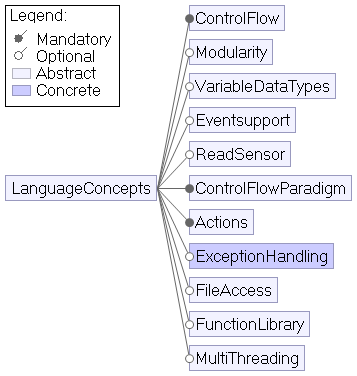
\includegraphics[width=\columnwidth]{LanguageConcepts.png}
      \caption{Language Concepts}
      \label{fig:langconcepts}
   \end{figure}

\parhead{Control Flow} - The languages typically offer several kinds of control-flow statements, such as, conditional structures (\texttt{if-do, if, if-else} and switch) loops (\texttt{do-while, while, forever, repeat while, repeat until}), and  interrupts (\texttt{loop interrupt} in \lego, \texttt{stop all} in \tello, \texttt{wait (time/event), break, and until}).
%\claudio{Use special font, e.g., texttt}
Multi-threading controls might be found also in \trik (\texttt{fork, join, kill thread}) and in  \lego for running tasks simultaneously (\texttt{sequence plug exit}).

\parhead{Modularity} - Modularity focuses at mission sub-components that are used to accomplish specific tasks.
Examples include \metabot, \ardublockly, \openroberta, \choregraphe, \sphero, \robotmesh, \metabot, \makeblock, \ozoblockly, and \turtlebot; they create mission modules using functions and function calls. Choregraphe implements robot behaviors as boxes, which are connected in a flow chart to form a mission. \lego imports blocks from external environments that are compatible with \lego. \trik implements subprograms, functions, and module with symbolic icon of what these components do; in this way they become mission modules. \picaxe implements procedures of particular concepts, which then can be invoked and used.  \missionlab has predefined states used to build a state machine for a given mission. 

\parhead{Variable data types} - While \flyaq, \missionlab, \tivipe, and \trik do not have exclusive variable data types, the rest of the environments have primitive types and compound data types. The primitive types include integer, decimal, character, float, number, and boolean, while compound types include strings/text, arrays, table, and lists. Other types include sound in \ozoblockly, logic (true, false) in \lego, degrees in \tello, and color in \sphero. In \aseba, state is a variable type;  for instance temperature is a variable that can take values like off, low, medium, high, and light is a variable that can take values like on and off. 

\parhead{Function libraries} - Function libraries offer functions and operation on data, including complex algorithms used to process data. Most environments provide function libraries for mathematics, logic and string operation; however \missionlab, \flyaq, \aseba, \codelab, and \tello do not offer such libraries. 

%\parheadit{Examples}
Top provide some examples, the logic functions include comparison like and/or, not, true/false, null, and test. The math sub-feature includes mathematics function, calculating parameters, trigonometric function, constant, number property, change by x, round, list evaluation, remainder of, constrain, random (integer, fraction), squareroot, return constant(sqrt, pi,...), sum of list, array operations, and range. Text operations include create, append, build string, length, find occurrence in a list, get sublist, is empty, get letter, get substring, join, and letter 1 of.  %Math box and data edit box in \choregraphe.     

\parhead{Control flow paradigm} - This determines how missions are executed, which can take the form of imperative execution, reactive paradigm or goal based. In imperative execution, the mission runs in the order of sequence of the tasks specified, which is the common paradigm of most environments in this study. However, \aseba Visual Programming features a reactive paradigm in which events, which act as triggers are matched with corresponding actions, which categorize it as a reactive. In some of the imperative environments like \picaxe, reactive aspects are also realized as robot, which responds to sensor data during mission execution. We did not come across an environment, which follows a goal-based control-flow paradigm.

 
\parhead{Actions} - These are activities robots execute to achieve a given task. Some are reactions to events, while others are activities that are imperatively specified in the mission. We classified robot actions as action type, actuation action, communication action, and movement actions. Robot actions  can be instantaneous actions e.g. take photo~\cite{FLYAQ}, pause, resume~\cite{PICAXE}, or continuous action e.g. follow line~\cite{LEGO,Sphero}, or timed executions where duration of execution is measured with start/stop time or events, like record a video~\cite{FLYAQ}. The actuation actions refer to device/actuator wise actions like grasp an object, motor movements, audio play. Communication actions include interacting with humans and non-human agents.  Communication with humans can be of the form of text, video, or audio. While non-human agents can  be categorized as tuple space, publish-subscribe or message passing. Tuple space is a shared space where shared data items are kept for access to entities entitled to access them, publish-subscribe where publishers avail messages regardless of receivers while subscribers receive messages they have subscribed to.
Movement actions manage mobility of robots. Languages offer concepts that specify how a robot moves from one location to another. Such  concepts are either absolute ``map coordinates", or relative like direction, distance, or travel time.\\
%\parheadit{Actuation examples identified} - 

Actuation examples include get button code, play tones, sound, stop motors, clear encoder, angular servo, turn on LED, detection with videocamera, line detector, video streaming enabling, beep note, buzzer, display, status light, object observation, taping, face status (smile, frown), lift, backpack, speak, think, change color, hide number, change volume, screen print, screen draw(line/object), start timer, set robot state, say hello, stand-up, wave with hand, move, DoPhoto, monitor street (road task), Intercept Object, LeaveRoom, Localize position, LookForObject, MarkNearestObject, MarkNearestDoor, MoveAhead, MoveAway, MOveForward, MoveToward, PickUp, SurveryRoom, Talk, Terminate, TrackTarget, Wait, Wander, follow line, gripper(open, close, stop), set mode(active, rest, sit). \patrizio{not sure we need all this}\\ 
 
%\parheadit{Action type examples}
Action type examples include the ``random eyes duration ms" block that is used in \openroberta to turn NAO's eye LEDS to change eye color for specified duration in milliseconds. Instead in NXT the ``get value ms timer" block is used as a sensor to read current time for another block, while the ``reset timer" block is used to reset the internal timer to zero. Similar time constructs also exist in other environment, like the wait time and elapsed time blocks in \ardublockly, the set roll time in seconds as a variable, time elapsed, get current time, set timeout, set time interval in \sphero, the set timer(seconds), timer, wait(seconds), wait until (event) in \vex among others. \\

%\parheadit{Communication examples} 
Communication example include infrared messages exchanged among robots in  \edison, \lego, and \openroberta, and Bluetooth messages exchange between bricks in Lego Ev3. In \missionlab, when in GOTO state, robots share information about target goal position and map of the environment among each other directly or through broadcasts. \sphero, \vex, \makeblock, and \tello broadcast message between robots. \flyaq supports synchronization and communication messaging among drones at run time.  \trik supports sending message to other robots. For what concerns human and central system to robot communications, examples are hand-clap and touch in \aseba, and \enchanting, send text, send number, send command, receive character, send character, send, and receive message in \tello, speak short phrase in \codelab, say text in \trik, \tivipe from the robot to the environment. In \choregraphe robot can share text with humans. In \arcbotics, humans interact with robot through beep, status led colors, infrared remote code and \picaxe communicates through infrared messages. Eleven of the 29 environments do not offer any communication language constructs. \\

%\parheadit{Movement examples} 
Few of the environments support absolute movement actions, such as e.g. goto (coordinates) in \flyaq, \missionlab, \makeblock, moveto (coordinates), movefast (coordinates, duration) in \tivipe, roll(angle, speed, time), spin(angle, time in seconds) in \sphero, drive (distance) in \codelab. For relative movements we mention go/move/drive/turn/fly (forward/backward/left/right/room) as seen in most of the environments like \metabot, \trik, and \lego.

\parhead{Event support} - Event support considers language abilities to handle events like creating event handlers, the types of events that can be recognized, and mechanisms of synchronizing events to subsequent actions. The common language constructs for event support identified include when (event), when (event) do, wait for (event), wait until (event), wait (event), on (event), capture(event), move until (event), broadcast and wait 9event) in \vex, AtGoal, AtEndOfHall, in \missionlab, and delay (event). The events are sensory data that trigger the next robot action. However environments like \arcbotics, \tivipe, \minibloq, \turtlebot, and \robotc do not have event support language constructs.\\

\parhead{Read Sensor} - From the environment the robot captures data through sensor readings, which inform robots next action. Much as most environments offered language support to capture respective sensor data, \turtlebot and \missionlab do not offer language concepts to manipulate sensors while \choregraphe supports vision recognition using vision reco box and sound recognition using speech reco box. \ozoblockly uses proximity sensor concept to detect objects without details of the sensor.\\

%\parheadit{Example} 
Common sensors captured in the environments include gyro for measuring rotations, light/light intensity, sound/clap detector, touch, temperature/thermometer, ultrasonic for measuring distance, timer, compass, accelerometer, gesture detector, and face recognizer. Other sensors are sonar, infrared ranger, GPS module, finger print scanner, motor rotation counter, energy meter, line detector, angle reader, line tracker, potentiometer, velocity, power(wats), current (amps), magnetometer, and force resister. The number of sensors on the robot and nature of the missions the robot is designed for determine the language constructs for the sensors.  \\

\parhead{Exception Handling} - Only three environments, namely \openroberta, \choregraphe, and \codelab offer support for exception handling in their text notation but none in the graphical notation. %\tb{probably just very few, right?} 

%\parheadit{Examples} 
More specifically, \openroberta exploits the Python exception handler, and \choregraphe exploits the try catch block for all errors in C++ software development kit (SDK) and the try catch block for face detection error in python SDK. \codelab offer support for exception handling for the following errors: actionerror, animations not loaded, can not place objects on this, connection aborted, connection check failed, connection error, no devices found, not pickupable, and robot busy.\\

\parhead{File Access} - It is a block found in \lego, used for reading and writing data from and to memory, close or delete a file. Such file can record for instance ambient light measurements taken at given time intervals, which are stored in memory and can be displayed on the LCD display screen ~\cite{LEGO}. \trik allows writing to robot file system, \choregraphe supports open, close and save operations to file while \missionlab offers read, write, close and delete language construct for file operations. \picaxe also supports read and write operations. The rest of the environments do not offer any language support for file access operations.

\parhead{Multithreading} - This concept when supported by a language enables users to do several activities without waiting for one activity to end. This improves speed of execution especially when it involves user. In \robotmesh,  using blockly editor,  \textit{start} block creates s thread, \textit{sleep} for x seconds forces thread to \textit{yield}, \textit{start autonomous} creates a thread that runs in autonomous mode of the robot, \textit{start driver} creates a thread that runs in driver mode. In python, sys.run\_in\_thread(f), sys.thread\_id(), sys.sleep(t). In C++, thread (void (*callback)(void)), get\_id(), join(), interrupt(), yield(), sleep\_for(unit32\_t time\_ms), lock(), try\_lock(), unlock(). \trik offers fork, join, kill thread, send message to thread functions to execute multithreading. \lego offers Sequence Plug Exit block for creating parallel tasks, though the simultaneous tasks need to be manually verified to avoid resource conflicts. \makecode and \robotc use \textit{run in parallel} block to support multithreading of mission tasks. \tivipe uses \textit{splitSCIS} to split and run three modules  in parallel. \missionlab supports Cthread, which is a lightweight process threads package from Georgia Tech which operates under Linux, SunOS operating systems. While \picaxe supports multi-tasking with operations like; restart, resume, and suspend.












  %\begin{figure}[h]
% \subsection{How the environments differ}
% \noindent
% General language features ~\cite{Clark}; notation is the concrete syntax of a language expressed either as textual syntax or visual syntax. Abstract syntax describes the vocabulary of the concept and how they are combined, while semantics describes what the language represents and means. Mapping feature describes how the language translates to other languages, its semantic equivalence, abstraction level with respect to similar languages and also internal mapping of the abstract syntax to concrete syntax as part of the language architecture. While extensibility of the language states how the language handles adding new concepts to boost its expressiveness. By considering features as end-user visible characteristics of the system, the environments can be compared based on; notation, extensibility, semantics and some aspects of mapping.
% Feature matrix\\
% $\bullet$ Notation matrix\\
% $\bullet$ coupling and reuse of mission artifacts in different contexts\\
% $\bullet$ control flow at run time; imperative (sequence and branch, in concurrent threads, reactive to events or declarative)\\
% editing features (syntax, semantic 

% What made the environments different\\
% $\bullet$ \parhead{Based on underlying technology} blockly based, scratch based, or generic \\
% $\bullet$ \parhead{Connection of blocks} flow chart based or nonflow chart (no links between blocks)\\
% $\bullet$ \parhead{Closeness of mapping} icon based or regular graphical blocks\\
% $\bullet$ \parhead{User domains} students focused (learning), electro-mechanical domain with features of electronics components like motors, programming domains demonstratting features of programming languages,\\ 
% $\bullet$ \parhead{Semantics} are the languages interpreted or compiled. The common generated code languages including; Java Script, Java, C/C++, Python.\\
% $\bullet$ \parhead{Control flow Vs Data flow based}. Control flow based languages graphical languages organize functional blocks into directed graph using arrows. A current block executes command and passes control to the next block based on the output generated. While in data flow based languages, program blocks are data variables that receive data from sensor system, whose value determines the next course of action ~\cite{Mordvinov2017}.
% ======================
% To be crosschecked~\cite{crosscheck}

% \begin{itemize}
% %In robotics, who specifies the mission requirements? (user domain expert, robotic engineer)
%     \item Task features; behavioral/functional model
%     \item Environmental features
%     \item Performance metrics; governing rules that constrain the behavior of the task
%     \item Robot capabilities; physical parts(actuators) that exhibit the behavior of the task
%     \item Mission goal; user goal, purpose of the mission
%     \item Single robot or team of robots mission, if multi-robots, the task distribution/delegation strategy (automatic or explicitly specified).This also includes interactive missions where humans work with robots.
%     \item In quantitative specifications, execution times for respective tasks should be specified otherwise sequence of specification for qualitative specifications.This can be an input to motion planning unit.
%      \item Text; type or select from drop-down list
%     \item Visual/graphical; point at locations to visit in a map, drag and drop domain primitive icons to define sequence of events.
%     \item Audio interaction with robot
%     \item task specification tree where nodes are declarative specification of tasks to perform\cite{Doherty2013}. Can missions be decomposed to tasks and subtasks to form a task forest or bigger tree? Weintrop et al \cite{Weintrop2018} reports use of trees to hierarchically program tasks. Robot routine is broken  into  a series of steps, with each step having sub steps, resulting into hierarchical program as implemented in universal robots' polyscope interface.
% \end{itemize} 
% \claudio{Can you try to put here for each RQ the concepts that aims at answering that RQ. For example, 
% RQ1: Debugging, Simulator.}
% \claudio{If you collected something that is not mapped to an RQ you have two options:
% 1 - you drop it. Because the information is not useful
% 2 - you add a new RQ.}